% !TeX spellcheck = en_GB

\section{Introduction into Building Automation}
\label{sec:background:bas:intro}

\begin{comment}
		\begin{itemize}
		\item Increasing amount of complexity and requirement of comfort in private and commercial buildings \parencite{Merz2009}

		\item benefits regarding saving and managing energy \parencite{Merz2009}
		\item Ever changing requirements: "in commercial buildings flexibility is high on the agenda -- offices buildings, for example, should be designed in such way that they can be easily adapted to meet any change in use or requirements" \parencite{Merz2009}
		\item "In modern buildings there are variety of automation systems for heating, ventilating and air conditioning" \parencite{Merz2009}
		\item "control systems optimize energy consumption and enable support and maintenance personnel to carry out their jobs more efficiently" \parencite{Merz2009}
		
	\end{itemize}
\end{comment}

With the ever increasing amount of requirements and complexity with regards to lighting, \gls{hvac} in private and commercial buildings, more versatile and flexible wiring and control solutions are required. 
Additionally, more flexible solutions offers possibilities like comfort functions, increased energy efficiency, and ease of maintenance. \parencite{Merz2009}

This solutions is offered by modern building automation systems and networks. Especially in commercial buildings requirements to rooms might change regularly, and hence they should be designed to accommodate these changes. \parencite{Merz2009}

\todo{more?}

% ------------------------------------------------------------------------------
\section{KNX}
\label{sec:background:bas:knx}

\alert{telegram vs frame. frame is used in the english standard document -> will use telegram}
\begin{comment}
	\begin{itemize}
		\item \knx or Konnex
		\item "formerly known as European Installation Bus (EIB)" \parencite{Merz2009}
		\item "designed to be used in electrical installations for implementing automated functions and processes in buildings" \parencite{Merz2009}
		\item "Different transmission media can be used for the bus: twisted-pair cable (KNX.TP), power line (KNX.PL), radio frequency (KNX.RF) and fiber-optic cable" \parencite{Merz2009}
		\item focus on KNX.TP
			\subitem 2 variants
			\subitem TP-0: 2400 Baud unbalanced, derived from BatiBUS \parencite{CENELEC2004} \parencite{DIN_EN_50090-5-2}
			\subitem TP-1: 9600 Baud balanced, derived from EIB (relevant here) \parencite{CENELEC2004} \parencite{DIN_EN_50090-5-2}
		\item KNX.PL and KNX.RF for integration into older buildings \parencite{Merz2009}
		\item Standardized as DIN EN 50090 written by \textcite{CENELEC2004} \parencite{DIN_EN_50090-5-2}
		\item "Large sections was approved for inclusion into ISO/IEC 14543" \parencite{Merz2009}
		\item "World wide only open standard for home and building control" \parencite{Merz2009}
		\item Benefits of \knx include
			\subitem more devices due to different manufactures
			\subitem large variety of devices (sensors, actuators, control/regulation, operation and monitoring)
	\end{itemize}
\end{comment}

One of most commonly used systems for building automation systems in Germany and Europe is \Gls{knx} or Konnex. Formerly known as the \gls{eib}, \gls{knx} is a \alert{conglomerate} of multiple building automation vendors, resulting in the KNX Association. \todo{link as footnote?}
It was designed to substitute traditional electrical installations and to implement functions and processes in an automated fashion. \parencite{Merz2009}

\Gls{knx} protocol is defined in the DIN EN 50090 family and can the transmitted over various physical media. Among those physical layers are \gls{knx} over twisted pair (KNX.TP), \gls{knx} over power line (KNX.PL) and \gls{knx} over radio (KNX.RF). Later 2 are intended for retrofitting older buildings. \parencite{Merz2009}
\alert{forgot KNX/IP}

As a result, \gls{knx} twisted-pair is the most commonly used installation method and is defined in 2 flavours. \parencite{DIN_EN_50090-5-2}
The older variant TP-0 was derived from the BatiBUS \todo{ref?} and operates at 2400 Baud. However, nowadays most \gls{knx} devices implement TP-1, operating at 9600 Baud, which is a direct successor of \gls{eib}.

One of the most appealing benefits of using \gls{knx} is the ubiquitous availability as world wide accepted DIN standard, which was even amplified as large sections were included in ISO/IEC 14543.
Following, more devices from multiple vendors are available with a large variety of sensors, actuators, control and regulation solutions, as well as operation and monitoring.

From an academic point of view the easy availability of the standards, provides a good understanding of the protocol. Therefore allowing for analysis without prior reverse-engineering the protocol.
Additionally the University of Rostock also uses \gls{knx} in some buildings \todo{ref to Thomas}, which provides an promising source of test and demo data.

% ------------------------------------------------------------------------------
\subsection{Bus Topology of KNX Networks}
\label{sec:background:bas:knx:topo}

\begin{comment}
		\begin{itemize}
		\item "Like a conventional electrical installation, a KNX installation needs to have a power line network to provide the loads with electricity. But it also has a communication network – the KNX installation bus" \parencite{Merz2009}
		\item "Both networks are galvanically isolated" \parencite{Merz2009}
		\item 2 separate cable installations as a result
		\item \knx is designed to reshape the structure of conventional building installations, in form of a tree topology \parencite{Merz2009}
		\item "Nodes are assigned to a line" \parencite{Merz2009}
		\item "Several lines are connected to a main line and form an area" \parencite{Merz2009}
		\item "Several areas are connected with each other via the back bone line" \parencite{Merz2009}
		\item Each node is assigned an address, defining area, line, and device number which forms the logical topology
			\subitem cf. Table~\ref{tab:background:bas:knx:topo:addr}
		\item It is advised, that the physical topology reassembles the logical \parencite{Sokollik2017}
		\item Even though, the physical \knx bus can build in various forms (star, tree, and mixed forms) \parencite{Sokollik2017}
		\item Most significant subdivision of the physical topology in \knx.TP-1 is a line segment \parencite{Sokollik2017}
			\subitem a segment defines how many \knx devices can be connected on a physical line \parencite{Sokollik2017}
			\subitem segment is a part of the bus system, which connects \knx devices electrical continuous with each other. \parencite{Sokollik2017}
		\item 2 types of \knx.TP-1 devices \parencite{Sokollik2017}
			\subitem TP1-64 and TP1-256 cf. Table \ref{tab:background:bas:knx:topo:tpsegments}
			\subitem mainly differ in the maximum amount of devices, which can be connected in one segment
			\subitem problem since market is very fragmented
			\subitem products are often not clearly with regards to TP1-64 and TP1-256
			\subitem better of assuming TP1-64 for installations, since one TP1-64 device in a segment forces the whole segment to be downgraded to the TP1-64 standard
		\item therefore max a full logical line must be build in four segments with 3 line repeaters \parencite{Sokollik2017}
			\subitem it is to note that is not to advice since a \knx telegram can only take 6 hops
			\subitem e.g. can be transmitted by max 6 couplers
		\item area is created by coupling up to 16 lines \parencite{Sokollik2017}
			\subitem 1 main line and 15 sublines
			\subitem lines are coupled via line couplers to the main line
			\subitem line couplers have own physical address (device address 0) \parencite{Sokollik2017}
			\subitem line couplers galvanically separate main line and sub line, are capable of routing \parencite{Sokollik2017}
		\item all main lines are connected via backbone couplers to the backbone line \parencite{Merz2009}
	\end{itemize}
\end{comment}

To accommodate for the initially mentioned advanced features in building automation systems, like central control and management, improved energy efficiency, or other comfort functions \gls{knx} introduces an additional wiring installation (cf. Section~\ref{sec:background:bas:knx}) next to the conventional mains power line. Both of these installations are galvanically isolated and \gls{knx} merely use mains power for actuators e.g. lights or blinds, since the \gls{knx} devices are powered via the \gls{knx} bus from special \gls{knx} power supply units containing a choke. \hint{Maybe explain this?} Each power supply is able to power up to 32 or 64 devices, depending on the model.
As a result, 2 separate cable installations are required.
Besides the physical \gls{knx} wiring can be constructed in various forms, like star, tree, or mixed forms, it is strongly advised to ensure that the physical wiring resembles the logical structure of the network. \parencite{Sokollik2017,Merz2009}
\todo{write about more about physical installation of knx?}

The logical structure builds on top of the physical topology and is intended to remodel the functional structure of buildings in a logical tree topology. This tree topology is divided into 3 levels: areas, lines, and devices. Each device or node is assigned a physical address, defining area, line, and device number. (cf. Table~\ref{tab:background:bas:knx:topo:addr})
Each device is directly connected to a line, which can accommodate up to 256 devices, if supported by all devices on the line. Alternatively, up to 64 devices can be in one line segment before line repeater is required. (cf. Table~\ref{tab:background:bas:knx:topo:tpsegments}
Most \gls{knx} devices still follow the TP1-64 specification and due to the high market fragmentation devices are often not mark in regards of supporting either TP1-64 or TP1-256, therefore it is still recommended to only use 64 devices within a line segment. \alert{sentence too long?} Thus, a full logical line is advised to be build using 3 line repeater. \parencite{Sokollik2017,Merz2009}

Usually a line coupler is installed as a line repeater. A line coupler is an active device to connect one logical level of the \gls{knx} network to another one, which can be one line segment to another line segment.
However, their original purpose is to separate the different levels of the logical \gls{knx} topology, explicitly to attach a line to the main line of an area or to attach a main line to the backbone. (cf. Figure~\ref{fig:background:knx:topo})
An area is formed by combining up to 16 lines: 1 main line and 15 sublines. All main lines are then connected to a backbone line, again via line couplers. \parencite{Sokollik2017}

As an active device line couplers are assigned an address, and is able to filter traffic by addresses similar to IP router. %usually with device number 0 in case it connects a line to backbone line.
Further couplers provide galvanic isolation, to mitigate damages by high voltages, shorts, etc. As a result multiple power supplies are required, basically one for each line segment.
An important feature to be aware of, when using line couplers, is that a \gls{knx} telegram can only be routed over 6 hops. This was introduced to prevent high network load in case of cyclic routing, comparable to the time to live in IP based networks. \parencite{Sokollik2017}

Additional to the physical address each devices is assigned, devices may listen to group addresses.
\todo{describe layers/modes of group addresses?}
Whereby physical addresses are used to communicate with one specific device, which is common during installation, throughout normal operation mostly group addresses are used. As the name implies multiple devices may listen to such an address, allowing one light switch to turn on or off multiple lights for instance.

\hint{Move addressing into own subsection?}

\begin{figure}
	\centering
	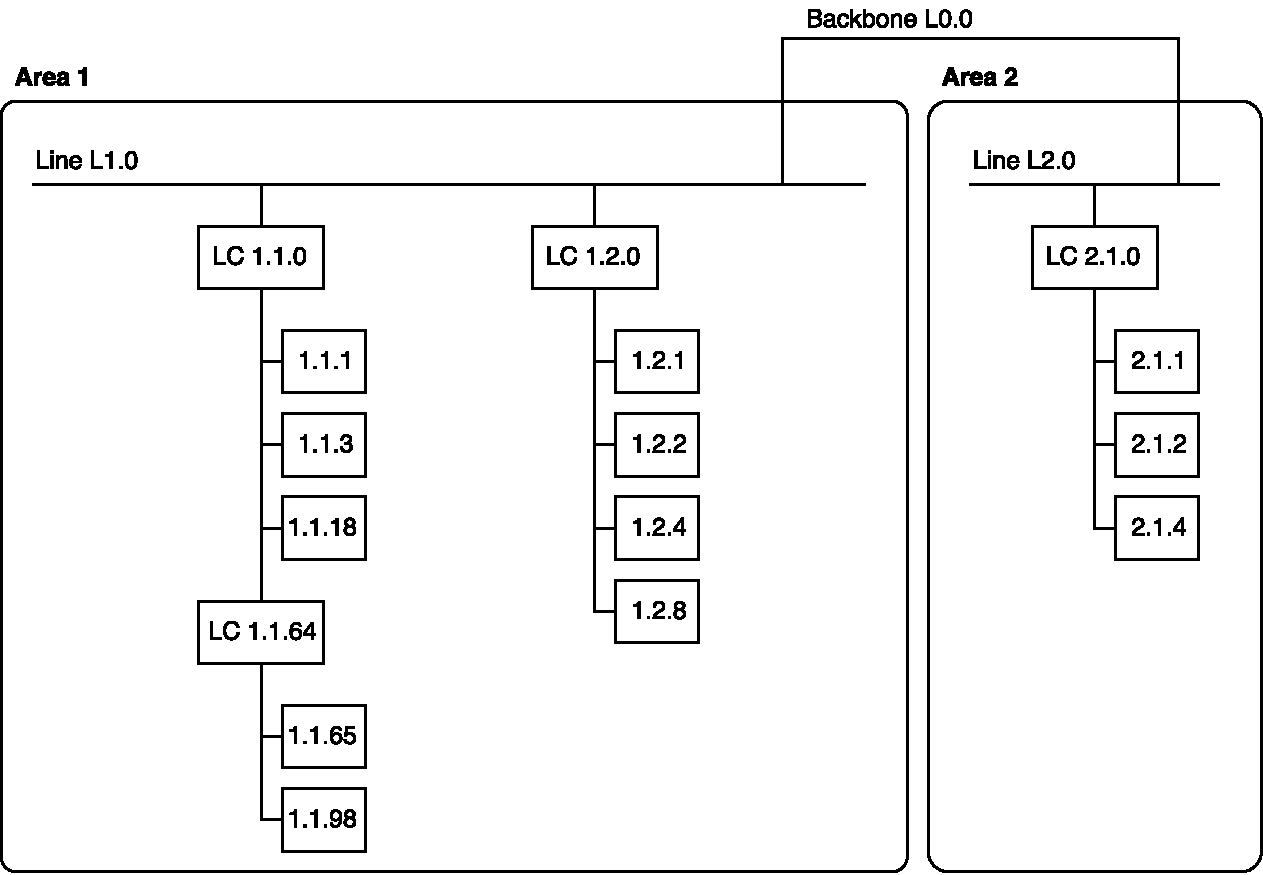
\includegraphics[width=\textwidth]{figures/100-knx-demo-topo.pdf}
	\caption[KNX network topology]{Exemplary logical topology of a \gls{knx} network with line couplers (LC) and normal devices. \todo{draw more nodes?} \todo{add LC for coupling to backbone} \todo{mark main line}}
	\label{fig:background:knx:topo}
\end{figure}
	
\begin{table}
	\aboverulesep=0ex
	\belowrulesep=0ex
	\renewcommand{\arraystretch}{1.2}
	
	\centering
	\begin{tabular}{|l|c|c|c|c|c|c|c|c|c|c|c|c|c|c|c|c|}
		\toprule
		Byte & \multicolumn{8}{c|}{1} & \multicolumn{8}{c|}{0} \\\midrule
		Bit & 7 & 6 & 5 & 4 & 3 & 2 & 1 & 0 & 7 & 6 & 5 & 4 & 3 & 2 & 1 & 0\\\midrule
		Physical Address & \multicolumn{4}{c|}{area} & \multicolumn{4}{c|}{line} & \multicolumn{8}{c|}{device}\\\midrule
		Group Address & \multicolumn{5}{c|}{main} & \multicolumn{3}{c|}{middle} & \multicolumn{8}{c|}{sub group}\\
		\bottomrule
	\end{tabular}
	\caption[Bit field for \knx addresses]{Bit field for \knx addresses. Only the most common used 3-level group address is shown here. cf.~\textcite{Merz2009,Sokollik2017} }
	\label{tab:background:bas:knx:topo:addr}
\end{table}

\begin{table}
	\centering
	\begin{tabular}{l r r }
	 & \textbf{TP1-64} & \textbf{TP1-256} \\\toprule
	 maximum devices per segment & 64 & 256 \\
	 maximum distance between 2 devices & 700m & 700m \\
	 maximum length of a physical line & 1000m & 1000m \\
	 \bottomrule
	\end{tabular}
	\caption[Segment properties for \knx.TP1-64 and \knx.TP1-256]{Segment properties for \knx.TP1-64 and \knx.TP1-256. cf. \textcite{Sokollik2017} \todo{adjust design of this table}}
	\label{tab:background:bas:knx:topo:tpsegments}
\end{table}

% ------------------------------------------------------------------------------	
\subsection{KNX Protocol}
\label{sec:background:bas:knx:proto}

\begin{comment}
		\begin{itemize}
		\item 3 types of telegrams \parencite{Hubner2009} \parencite{Merz2009}
			\subitem data - "sent in response to an individual action such as" \parencite{Merz2009} pressing a button (standard and extended \parencite{Hubner2009})
			\subitem acknowledge - "All devices (receivers) that belong to this group simultaneously confirm that they have received the data frame by returning an acknowledgment frame." \parencite{Merz2009}
			\subitem poll - "one device can query 1-Byte-Information from up to 15 other devices. Addressing is done via group addresses" \parencite{Hubner2009}
		\item Standard Data Telegram
			\subitem cf. Table~\ref{tab:background:bas:knx:proto:knx-standard}
		\item Extended Data Telegram
			\subitem cf. Table~\ref{tab:background:bas:knx:proto:knx-extended}
		\item Poll Telegram
			\subitem cf. Table~\ref{tab:background:bas:knx:proto:knx-poll}
		\item Acknowledge Telegram
			\subitem cf. Table~\ref{tab:background:bas:knx:proto:ack}
	\end{itemize}
\end{comment}

Within the \gls{knx} specification 3 types of telegrams are defined: Data Telegrams, Poll Telegrams, and Acknowledge Telegrams. (cf. Table~\ref{tab:background:bas:knx:proto:knx-standard},~\ref{tab:background:bas:knx:proto:ctrle},~\ref{tab:background:bas:knx:proto:knx-poll}, and~\ref{tab:background:bas:knx:proto:ack})
\todo{write about prio}

\begin{table}
	\aboverulesep=0ex
	\belowrulesep=0ex
	\renewcommand{\arraystretch}{1.2}
	\newcolumntype{Y}{>{\centering\arraybackslash}X}
	
	\centering
	\begin{tabularx}{0.7\textwidth}{|l|Y|Y|}
		\toprule
		Bit & 1 & 0 \\\midrule
		Function & \multicolumn{2}{c|}{Priority} \\\bottomrule
		\toprule
		System priority & 0 & 0 \\\midrule
		Alarm priority & 1 & 0 \\\midrule
		High priority & 0 & 1 \\\midrule
		Low priority & 1 & 1 \\\bottomrule
	\end{tabularx}
	\caption[\knx priority encoding]{\knx priority encoding. cf.~\textcite{Merz2009}}
	\label{tab:background:bas:knx:proto:prio}
\end{table}

\subsubsection{Data Telegram}

The data telegram being utilised the most and used for transferring commands, state, and value changes, comes in 2 flavours.
The standard data telegram (cf. Table~\ref{tab:background:bas:knx:proto:knx-standard}) is able to transmit between 2 and 16 bytes per telegram. To transfer more data the extended data telegram (cf. Table~\ref{tab:background:bas:knx:proto:knx-extended}) can be utilised, which can transfer up to 255 bytes.
Both are sent in reaction of an direct interaction (e.g. light switch) or to send periodical sensor data (e.g. temperature). \parencite{Merz2009}
The recipient answers then with an acknowledge telegram. \parencite{Merz2009,Sokollik2017}

\begin{table}
	\aboverulesep=0ex
	\belowrulesep=0ex
	\renewcommand{\arraystretch}{1.2}
	\newcolumntype{Y}{>{\centering\arraybackslash}X}
	
	\centering
	\begin{tabularx}{\textwidth}{|l|Y|Y|Y|Y|Y|Y|Y|Y|Y|Y|Y|Y|Y|Y|Y|Y|Y|Y|Y|Y|Y|Y|Y|Y|}
		\toprule
		Byte & \multicolumn{8}{c|}{0} & \multicolumn{8}{c|}{1} & \multicolumn{8}{c|}{2} \\\midrule
		Bit & & & & & & & & & & & & & & & & & & & & & & & & \\\midrule
		Function & \multicolumn{8}{c|}{CTRL} & \multicolumn{16}{c|}{Source Address} \\\bottomrule
		\toprule
		Byte & \multicolumn{8}{c|}{3} & \multicolumn{8}{c|}{4} & \multicolumn{8}{c|}{5} \\\midrule
		Bit & & & & & & & & & & & & & & & & & & & & & & & & \\\midrule
		Function & \multicolumn{16}{c|}{Destination Address} & \multicolumn{1}{c|}{\parbox[t][26pt][s]{0.2cm}{A T}} & \multicolumn{3}{c|}{Hops} & \multicolumn{4}{c|}{Length} \\\bottomrule
		\toprule
		Byte & \multicolumn{8}{c|}{6} & \multicolumn{8}{c|}{$7+n$} & \multicolumn{8}{c|}{$8+n$} \\\midrule
		Bit & & & & & & & & & & & & & & & & & & & & & & & & \\\midrule
		Function & \multicolumn{16}{c|}{Payload $n+1$ Bytes} & \multicolumn{8}{c|}{Parity} \\\bottomrule
	\end{tabularx}
	\caption[Standard \knx data telegram]{Standard \knx data telegram with $2$ to $16$ bytes of payload. Control Byte (CTRL) cf. Table~\ref{tab:background:bas:knx:proto:ctrl}, Source Address, Destination Address cf. Table~\ref{tab:background:bas:knx:topo:addr}, Address Type (AT), Hop Count (Hops), Payload Length (Length), Payload, and Parity.}
	\label{tab:background:bas:knx:proto:knx-standard}
\end{table}

\begin{table}
	\aboverulesep=0ex
	\belowrulesep=0ex
	\renewcommand{\arraystretch}{1.2}
	\newcolumntype{Y}{>{\centering\arraybackslash}X}
	
	\centering
	\begin{tabularx}{\textwidth}{|l|Y|Y|Y|Y|Y|Y|Y|Y|Y|Y|Y|Y|Y|Y|Y|Y|Y|Y|Y|Y|Y|Y|Y|Y|}
		\toprule
		Byte & \multicolumn{8}{c|}{0} & \multicolumn{8}{c|}{1} & \multicolumn{8}{c|}{2} \\\midrule
		Bit & & & & & & & & & & & & & & & & & & & & & & & & \\\midrule
		Function & \multicolumn{8}{c|}{CTRL} & \multicolumn{8}{c|}{CTRLE} & \multicolumn{8}{c|}{Source Address} \\\bottomrule
		\toprule
		Byte & \multicolumn{8}{c|}{3} & \multicolumn{8}{c|}{4} & \multicolumn{8}{c|}{5} \\\midrule
		Bit & & & & & & & & & & & & & & & & & & & & & & & & \\\midrule
		Function & \multicolumn{8}{c|}{Source Address} & \multicolumn{16}{c|}{Destination Address} \\\bottomrule
		\toprule
		Byte & \multicolumn{8}{c|}{6} & \multicolumn{8}{c|}{$7$} & \multicolumn{8}{c|}{$8+n$} \\\midrule
		Bit & & & & & & & & & & & & & & & & & & & & & & & & \\\midrule
		Function & \multicolumn{8}{c|}{Length} & \multicolumn{16}{c|}{Payload $n+1$ Bytes} \\\bottomrule
		\toprule
		Byte & \multicolumn{8}{c|}{$9+n$} & \multicolumn{16}{c|}{ } \\\cmidrule{1-9}
		Bit & & & & & & & & & \multicolumn{16}{c|}{ } \\\cmidrule{1-9}
		Function & \multicolumn{8}{c|}{Parity} & \multicolumn{16}{c|}{ } \\\bottomrule
	\end{tabularx}
	\caption[Extended \knx data telegram]{Extended \knx data telegram with $2$ to $255$ bytes of payload. Control Byte (CTRL) cf. Table~\ref{tab:background:bas:knx:proto:ctrl}, Extended Control Byte (CTRLE) cf. Table~\ref{tab:background:bas:knx:proto:ctrle}, Source Address, Destination Address cf. Table~\ref{tab:background:bas:knx:topo:addr}, Payload Length (Length), Payload, and Parity.}
	\label{tab:background:bas:knx:proto:knx-extended}
\end{table}

\begin{table}
	\aboverulesep=0ex
	\belowrulesep=0ex
	\renewcommand{\arraystretch}{1.2}
	\newcolumntype{Y}{>{\centering\arraybackslash}X}
	
	\centering
	\begin{tabularx}{\textwidth}{|l|Y|Y|Y|Y|Y|Y|Y|Y|}
		\toprule
		Byte & \multicolumn{8}{c|}{0} \\\midrule
		Bit & 7 & 6 & 5 & 4 & 3 & 2 & 1 & 0 \\\midrule
		Function & \multicolumn{2}{c|}{TT} & R & A & \multicolumn{2}{c|}{P} & \multicolumn{2}{c|}{reserved} \\\bottomrule \toprule
		Standard Data Telegram & 1 & 0 & R & 1 & \multicolumn{2}{c|}{P} & \multicolumn{2}{c|}{ } \\\midrule
		Extended Data Telegram & 0 & 0 & R & 1 & \multicolumn{2}{c|}{P} & \multicolumn{2}{c|}{ } \\\midrule
		Poll Telegram & 1 & 1 & 1 & 1 & 0 & 0 & \multicolumn{2}{c|}{ } \\\midrule
		Acknowledge Telegram & \multicolumn{2}{c|}{ } & 0 &0 & \multicolumn{2}{c|}{ } & \multicolumn{2}{c|}{ } \\\bottomrule
	\end{tabularx}
	\caption[\knx CTRL Byte]{\knx CTRL Byte. Telegram Type (TT), Repeat (R), Acknowledge (A), and Priority (P). cf. \textcite{Sokollik2017}}
	\label{tab:background:bas:knx:proto:ctrl}
\end{table}

\begin{table}
	\aboverulesep=0ex
	\belowrulesep=0ex
	\renewcommand{\arraystretch}{1.2}
	\newcolumntype{Y}{>{\centering\arraybackslash}X}
	
	\centering
	\begin{tabularx}{0.7\textwidth}{|l|Y|Y|Y|Y|Y|Y|Y|Y|}
		\toprule
		Byte & \multicolumn{8}{c|}{0} \\\midrule
		Bit & 7 & 6 & 5 & 4 & 3 & 2 & 1 & 0 \\\midrule
		Function & AT & \multicolumn{3}{c|}{Hops} & \multicolumn{4}{c|}{EFF} \\\bottomrule
	\end{tabularx}
	\caption[\knx CTRLE Byte]{\knx CTRLE Byte. Address Type (AT), Hop Count, and Extended Frame Format (EFF). cf. \textcite{Sokollik2017}}
	\label{tab:background:bas:knx:proto:ctrle}
\end{table}

\subsubsection{Acknowledge Telegram}

The acknowledge telegram can indicate the correct reception (\code{ACK}, positive acknowledge), faulty reception (\code{NACK}, negative acknowledge), or that the receiving device is currently busy and is not able to process the telegram. (cf. Table~\ref{tab:background:bas:knx:proto:ack})
It consists of 1 byte and is sent by the recipient after waiting 13 bit times.
If the sender receives an positive acknowledge, the telegram was send successfully and no further action is required. However, if it detects an negative acknowledge or busy signal, the telegram is resend up to 3 times.
Supposed a busy signal occurred, the sender adds a waiting period before attempting to resend the telegram.
Given, the sender does not receives any form of acknowledge telegram within 13 bit times, it resends the telegram also up to 3 times.
In case the sender addressed the original telegram to multiple devices by using a group address as destination, the acknowledge frame is send simultaneously by all recipients. Due to the bus characteristic of being normally high (1), an negative acknowledge or busy signal overrules a positive acknowledge, since \code{BUSY} and \code{NACK} are encoded with low bits (0). \parencite{Merz2009,Sokollik2017}

\begin{table}
	\aboverulesep=0ex
	\belowrulesep=0ex
	\renewcommand{\arraystretch}{1.2}
	\newcolumntype{Y}{>{\centering\arraybackslash}X}
	
	\centering
	\begin{tabularx}{0.7\textwidth}{|l|Y|Y|Y|Y|Y|Y|Y|Y|}
		\toprule
		Byte & \multicolumn{8}{c|}{0} \\\midrule
		Bit & 7 & 6 & 5 & 4 & 3 & 2 & 1 & 0 \\\bottomrule
		\toprule
		ACK  & 1 & 1 & 0 & 0 & 1 & 1 & 0 & 0 \\\midrule
		NACK & 0 & 0 & 0 & 0 & 1 & 1 & 0 & 0 \\\midrule
		BUSY & 1 & 1 & 0 & 0 & 0 & 0 & 0 & 0 \\\midrule
		NACK + BUSY & 0 & 0 & 0 & 0 & 0 & 0 & 0 & 0 \\\bottomrule
	\end{tabularx}
	\caption[\knx acknowledge telegram]{\knx short acknowledge telegram.}
	\label{tab:background:bas:knx:proto:ack}
\end{table}

\subsubsection{Poll Telegram}

The poll telegram allows to poll 1 byte of data from up to 15 devices, however, it is seldom used in \gls{knx} networks. It consists of a poll data request frame (cf. Table~\ref{tab:background:bas:knx:proto:knx-poll}) and a poll data response frame. Former starts the poll telegram and sets the group address to query, also it defines how many bytes to receive.
The poll data response consists of each device sending one byte on the bus without starting a new telegram. The responding devices are doing so in a prior configured time slot. \parencite{Hubner2009,DIN_EN_50090-5-2}

\begin{table}
	\aboverulesep=0ex
	\belowrulesep=0ex
	\renewcommand{\arraystretch}{1.2}
	\newcolumntype{Y}{>{\centering\arraybackslash}X}
	
	\centering
	\begin{tabularx}{\textwidth}{|l|Y|Y|Y|Y|Y|Y|Y|Y|Y|Y|Y|Y|Y|Y|Y|Y|Y|Y|Y|Y|Y|Y|Y|Y|}
		\toprule
		Byte & \multicolumn{8}{c|}{0} & \multicolumn{8}{c|}{1} & \multicolumn{8}{c|}{2} \\\midrule
		Bit & & & & & & & & & & & & & & & & & & & & & & & & \\\midrule
		Function & \multicolumn{8}{c|}{CTRL} & \multicolumn{16}{c|}{Source Address} \\\bottomrule
		\toprule
		Byte & \multicolumn{8}{c|}{3} & \multicolumn{8}{c|}{4} & \multicolumn{8}{c|}{5} \\\midrule
		Bit & & & & & & & & & & & & & & & & & & & & & & & & \\\midrule
		Function & \multicolumn{16}{c|}{Destination Address} & \multicolumn{4}{c|}{ } & \multicolumn{4}{c|}{poll data} \\\bottomrule
		\toprule
		Byte & \multicolumn{8}{c|}{6} & \multicolumn{16}{c|}{ } \\\cmidrule{1-9}
		Bit & & & & & & & & & \multicolumn{16}{c|}{ } \\\cmidrule{1-9}
		Function & \multicolumn{8}{c|}{Parity} & \multicolumn{16}{c|}{ } \\\bottomrule
	\end{tabularx}
	\caption[\knx poll telegram]{\knx poll telegram. Control Byte (CTRL) cf. Table~\ref{tab:background:bas:knx:proto:ctrl}, Source Address, Destination Address cf. Table~\ref{tab:background:bas:knx:topo:addr}, expected length of poll data (poll data), and Parity.}
	\label{tab:background:bas:knx:proto:knx-poll}
\end{table}

\subsection{\knx communication}
\label{sec:background:bas:knx:communication}

	\begin{itemize}
		\item application layer described in \textcite{DIN_EN_50090-4-1}
		\item communication modes \parencite{DIN_EN_50090-4-1}
			\subitem point-to-multipoint, connection-less (multicast)
			\subitem point-to-domain, connection-less (broadcast)
			\subitem point-to-all-points, connection-less (system broadcast)
			\subitem point-to-point, connection-less
			\subitem point-to-point, connection-oriented
		\item APCI describes operation on application layer
		\item Response need to match the Request APCI type and must be send on the corresponding communication mode allowed for this packet. cf. \textcite[][page 9--10]{DIN_EN_50090-4-1}
		\item 
	\end{itemize}
	
\subsubsection{Network management procedures}
	\begin{itemize}
		\item "describe the device independent management procedures" \parencite{DIN_EN_50090-7-1}
		\item "shall be used to configure the network, and to get the information about the configuration of the network and connected devices" \parencite{DIN_EN_50090-7-1}
		\item " no knowledge of the single devices is required. They will work with every device connected to the network" \parencite{DIN_EN_50090-7-1}
		\item "shall be based on the use of the dedicated application layer services which are specified in EN 50090-4-1 \parencite{DIN_EN_50090-4-1} for this purpose" \parencite{DIN_EN_50090-7-1}
	\end{itemize}
	
\subsection{Security in KNX}
	\begin{itemize}
		\item copulers allow filtering 
			\subitem "This means that data frames transmitted by a sender are only forwarded to recipients that are not on the sender’s line." \parencite{Merz2009}
			\subitem "The filter function only forwards data frames to where they are needed. This reduces the overall amount of data frame traffic and keeps the data traffic on one line separate from the data traffic on another line, allowing data to be transferred on several lines simultaneously." \parencite{Merz2009}
		\item main group 14 and 15 should not be used \parencite{Hubner2009}
			\subitem can not be filtered due to limited space for filter tables in couplers \parencite{Hubner2009}
			
			
	\end{itemize}

% ------------------------------------------------------------------------------
\subsection{Examples and Applications of KNX Networks}

\section{\lonworks}

\section{\bacnet}